\documentclass{beamer}
\usepackage[utf8]{inputenc}

\usetheme{Boadilla}
\usecolortheme{lily}
\usepackage{amsmath,amssymb,amsfonts,amsthm}
\usepackage{mathtools}
\usepackage{txfonts}
\usepackage{tkz-euclide}
\usepackage{listings}
\usepackage{adjustbox}
\usepackage{array}
\usepackage{tabularx}
\usepackage{lmodern}
\usepackage{gvv}
\usepackage{circuitikz}
\usepackage{tikz}
\usepackage{graphicx}

\setbeamertemplate{footline}
{
  \leavevmode%
  \hbox{%
  \begin{beamercolorbox}[wd=\paperwidth,ht=2.25ex,dp=1ex,right]{author in head/foot}%
    \insertframenumber{} / \inserttotalframenumber\hspace*{2ex} 
  \end{beamercolorbox}}%
  \vskip0pt%
}

\usepackage{tcolorbox}
\tcbuselibrary{minted,breakable,xparse,skins}




\providecommand{\nCr}[2]{\,^{#1}C_{#2}} % nCr
\providecommand{\nPr}[2]{\,^{#1}P_{#2}} % nPr
\providecommand{\mbf}{\mathbf}
\providecommand{\pr}[1]{\ensuremath{\Pr\left(#1\right)}}
\providecommand{\qfunc}[1]{\ensuremath{Q\left(#1\right)}}
\providecommand{\sbrak}[1]{\ensuremath{{}\left[#1\right]}}
\providecommand{\lsbrak}[1]{\ensuremath{{}\left[#1\right.}}
\providecommand{\rsbrak}[1]{\ensuremath{{}\left.#1\right]}}
\providecommand{\brak}[1]{\ensuremath{\left(#1\right)}}
\providecommand{\lbrak}[1]{\ensuremath{\left(#1\right.}}
\providecommand{\rbrak}[1]{\ensuremath{\left.#1\right)}}
\providecommand{\cbrak}[1]{\ensuremath{\left\{#1\right\}}}
\providecommand{\lcbrak}[1]{\ensuremath{\left\{#1\right.}}
\providecommand{\rcbrak}[1]{\ensuremath{\left.#1\right\}}}
\theoremstyle{remark}
\newcommand{\sgn}{\mathop{\mathrm{sgn}}}
\providecommand{\abs}[1]{\left\vert#1\right\vert}
\providecommand{\res}[1]{\Res\displaylimits_{#1}} 
\providecommand{\norm}[1]{\lVert#1\rVert}
\providecommand{\mtx}[1]{\mathbf{#1}}
\providecommand{\mean}[1]{E\left[ #1 \right]}
\providecommand{\fourier}{\overset{\mathcal{F}}{ \rightleftharpoons}}
%\providecommand{\hilbert}{\overset{\mathcal{H}}{ \rightleftharpoons}}
\providecommand{\system}{\overset{\mathcal{H}}{ \longleftrightarrow}}
	%\newcommand{\solution}[2]{\textbf{Solution:}{#1}}
%\newcommand{\solution}{\noindent \textbf{Solution: }}
\providecommand{\dec}[2]{\ensuremath{\overset{#1}{\underset{#2}{\gtrless}}}}
\newcommand{\myvec}[1]{\ensuremath{\begin{pmatrix}#1\end{pmatrix}}}
\let\vec\mathbf

\lstset{
%language=C,
frame=single, 
breaklines=true,
columns=fullflexible
}

\numberwithin{equation}{section}

\lstset{
  language=Python,
  basicstyle=\ttfamily\small,
  keywordstyle=\color{blue},
  stringstyle=\color{orange},
  numbers=left,
  numberstyle=\tiny\color{gray},
  breaklines=true,
  showstringspaces=false
}

\title{Problem 8.4.26}
\author{ee25btech11023-Venkata Sai}

\date{\today} 
\begin{document}

\begin{frame}
\titlepage
\end{frame}

\section*{Outline}
\begin{frame}
\tableofcontents
\end{frame}

\section{Problem}

\begin{frame}
\frametitle{Problem}
The locus of the mid-point of the line segment joining the focus to a moving point
on the parabola $y^2 = 4ax$ is another parabola with directrix
\begin{enumerate}
    \item $x=0$
    \item $x=-a/2$
    \item $x=a$
    \item $x=a/2$
\end{enumerate}
\end{frame}
%\subsection{Literature}
\section{Solution}

\subsection{Formula}
\setcounter{section}{1}
\begin{frame}
\frametitle{Formula}
The equation of a conic with directrix $\vec{n}^\top \vec{x} = c$, eccentricity $e$ and focus $\vec{F}$ is given
by
\begin{align}
  \vec{x}^\top\vec{V}\vec{x} + 2\vec{u}^\top\vec{x} + f &= 0 
\end{align}
On comparing with $y^2-4ax=0$
\begin{align}
    \vec{x}^\top\vec{V}\vec{x}&= y^2\\  
    \vec{x}^\top\vec{V}\vec{x}&= \sbrak{\myvec{0 &1}\vec{x}}^2 
    \end{align}
    \begin{align}
     \vec{x}^\top\vec{V}\vec{x}= \brak{\myvec{0 &1}\vec{x}}^\top\brak{\myvec{0 &1}\vec{x}}\end{align}
     \begin{align}
         \vec{x}^\top\vec{V}\vec{x}&= \vec{x}^\top\myvec{0 \\1}\myvec{0 &1}\vec{x}\\
         \vec{x}^\top\myvec{\vec{V-\myvec{0 &0\\0&1}}}\vec{x}&=0 \implies \vec{V}=\myvec{0 &0\\0&1}
     \end{align}
\end{frame}
\subsection{Locus}
\begin{frame}
\frametitle{Locus}
 \begin{align}
     2\vec{u}^\top\vec{x}&=-4ax\\
     2\vec{u}^\top\vec{x}=-4a\myvec{1 & 0}\vec{x} &\implies  2\vec{u}^\top\vec{x}=\myvec{-4a & 0}\vec{x}\\
     \brak{2\vec{u}^\top-\myvec{-4a & 0}}\vec{x}=0 &\implies \vec{u}^\top=\myvec{-2a & 0}\\
     \vec{u}&=\myvec{-2a\\0}\\
     f&=0\\
     \vec{F}&=\myvec{a\\0}
     \end{align}
     Let $\vec{X}$ be the point of locus of the midpoint
\begin{align}
    \vec{X}=\frac{\vec{x}+\vec{F}}{2}\implies
    \vec{x}=2\vec{X}-\vec{F}
\end{align}     

\end{frame}
\subsection{Simplify}
\begin{frame}
\frametitle{Simplify}
From \brak{1} and \brak{13}
 \begin{align}
  \vec{x}^\top\vec{V}\vec{x} &+ 2\vec{u}^\top\vec{x} + f = 0\\
 \brak{ \vec{2\vec{X}-\vec{F} }}^\top\vec{V}\brak{\vec{2\vec{X}-\vec{F} }}& + 2\vec{u}^\top\brak{\vec{2\vec{X}-\vec{F}} } + f = 0 \\
  \brak{ \vec{2\vec{X}^\top-\vec{F}^\top }}\vec{V}\brak{\vec{2\vec{X}-\vec{F} }} &+ 2\vec{u}^\top\brak{\vec{2\vec{X}-\vec{F}} } + f = 0 \\
4\vec{X}^\top\vec{V}\vec{X}-2\vec{X}^\top\vec{V}\vec{F}-2\vec{F}^\top\vec{V}\vec{X}&+\vec{F}^\top\vec{V}\vec{F}+4\vec{u}^\top\vec{X}-2\vec{u}^\top\vec{F}+f=0
  \end{align}
   As $\vec{V}$ is a symmetric matrix
  \begin{align}
4\vec{X}^\top\vec{V}\vec{X}-2\vec{F}^\top\vec{V}\vec{X}-2\vec{F}^\top\vec{V}\vec{X}+\vec{F}^\top\vec{V}\vec{F}+4\vec{u}^\top\vec{X}-2\vec{u}^\top\vec{F}+f=0 \\
4\vec{X}^\top\vec{V}\vec{X}-4\vec{F}^\top\vec{V}\vec{X}+4\vec{u}^\top\vec{X}+\vec{F}^\top\vec{V}\vec{F}-2\vec{u}^\top\vec{F}+f=0\\
\vec{X}^\top\brak{\vec{4V}}\vec{X}+2\brak{2\brak{\vec{u}^\top-\vec{F}^\top\vec{V}}}\vec{X}+\vec{F}^\top\vec{V}\vec{F}-2\vec{u}^\top\vec{F}+f=0\\
\vec{X}^\top\brak{\vec{4V}}\vec{X}+2\brak{2\brak{\vec{u}-\vec{V}\vec{F}}^\top}\vec{X}+\vec{F}^\top\vec{V}\vec{F}-2\vec{u}^\top\vec{F}+f=0
 \end{align}
 \begin{align}
 \vec{V}'=4\vec{V}=4\myvec{0& 0 \\0&1}&=\myvec{0&0\\0&4}
 \end{align}
 \end{frame}
 \subsection{Finding the variables}
\begin{frame}
\frametitle{Finding the variables}
\begin{align}
  \vec{u'}=2\brak{\vec{u}-\vec{V}\vec{F}}=2\brak{\myvec{-2a\\0}-\myvec{0&0\\0&1}\myvec{a\\0}}&=2\brak{\myvec{-2a\\0}-\myvec{0\\0}}   \nonumber \\
  &=\myvec{-4a\\0}
  \end{align}
  \begin{align}
  f'&=\vec{F}^\top\vec{V}\vec{F}-2\vec{u}^\top\vec{F}+f \\
  f'&=\myvec{a\\0}^\top\myvec{0&0\\0&4}\myvec{a\\0}-2\myvec{-2a\\0}^\top\myvec{a\\0}+0\\
  f'&=\myvec{a&0}\myvec{0&0\\0&4}\myvec{a\\0}-2\myvec{-2a&0}\myvec{a\\0}+0\\
  f'&=\myvec{0&0}\myvec{a\\0}-2\myvec{-2a&0}\myvec{a\\0}+0\\
  f'&=-2\brak{-2a^2}=4a^2
 \end{align}
 
\end{frame}
\begin{frame}
\subsection{Eigen vector}
\frametitle{Eigen vector}
Finding eigen values of $\vec{V'}$
 \begin{align}
         |\vec{V'}-\lambda\vec{I}|&=0\\
         \mydet{\myvec{0&0\\0&4}-\myvec{\lambda&0\\0&\lambda}}=0&\implies \mydet{-\lambda&0\\0& 4-\lambda}=0
     \end{align}
     \begin{align}
         \brak{-\lambda}\brak{4-\lambda}=0 \implies \lambda_1=0\ \text{and}\ \lambda_2=4
     \end{align}
$\vec{p_1}$ is an eigen vector of $\vec{V'}$
\begin{align}
   \brak{ \vec{\vec{V'}-\lambda\vec{I}}}\vec{p}=\vec{0}
\end{align}
From \brak{30} and substituting $\lambda$=0
\begin{align}
    \myvec{0&0\\0&4}\vec{p_1}=\myvec{0\\0}\implies
    \myvec{0&0\\0&4}\myvec{x\\y}=\myvec{0\\0} \\
    0=0,y=0 \implies \vec{p_1}=\myvec{1\\0}
\end{align}
\end{frame}
\begin{frame}
\frametitle{Conclusion}

 The Equation of a Directrix is given by
 \begin{align}
     \vec{n}^\top\vec{x}=c
 \end{align}
 where
 \begin{align}
     \vec{n}=\sqrt{\lambda_2}\vec{p_1}\ \brak{\text{and}}\ c=\frac{\brak{\norm{\vec{u'}}^2-\lambda_2f}}{2\vec{u'}^\top\vec{n}} \\
     \vec{n}=\sqrt{4}\myvec{1\\0} \implies \vec{n}=\myvec{2\\0} 
     \end{align}
     \begin{align}
     c=\frac{\brak{\brak{-4a}^2+\brak{0}^2-4\brak{4a^2}}}{2\myvec{-4a\\0}^\top\myvec{2\\0}}  =\frac{\brak{16a^2-16a^2}}{2\myvec{-4a\\0}^\top\myvec{2\\0}}  =0
 \end{align}
 From \brak{36}
 \begin{align}
     \myvec{2&0}\myvec{x\\y}=0 \implies 2x=0 \implies x=0
 \end{align}
\end{frame}
\subsection{Plot}
\begin{frame}[fragile]
\frametitle{Plot}

\begin{figure}[h!]
   \centering
   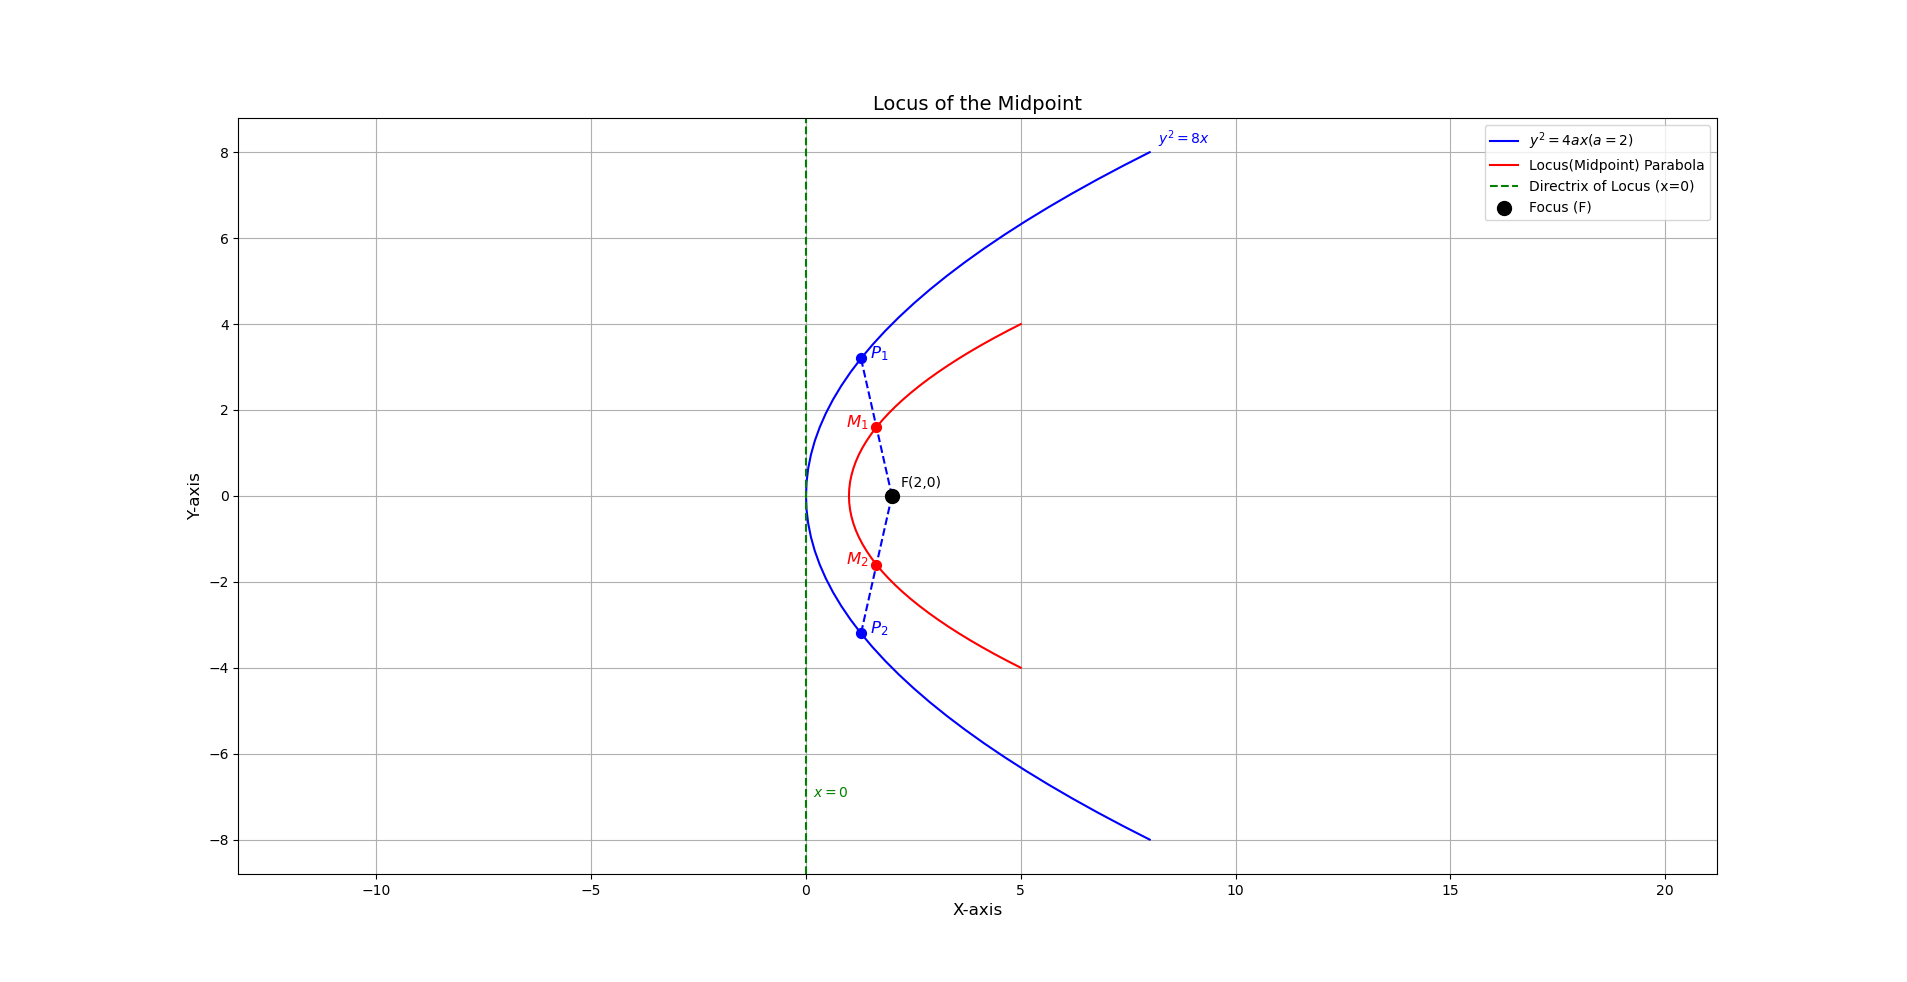
\includegraphics[width=1\columnwidth]{figs/fig1.png}
	\caption{}
   \label{}
\end{figure}
\end{frame}

\section{C Code}
\begin{frame}[fragile]
\frametitle{C Code}
\begin{lstlisting}[language=C]
void get_plot_data(double* out_data) {
    double a = 2.0;
    int num_points = 51;
    double t;
    out_data[0] = a;
    out_data[1] = 0.0;
    int index = 2;
    for (int i = 0; i < num_points; i++) {
        t = -2.0 + (4.0 * i) / (num_points - 1);
        out_data[index]     = a * t * t;
        out_data[index + 1] = 2 * a * t;
        out_data[index + (num_points * 2)]     = (a + a * t * t) / 2.0;
        out_data[index + (num_points * 2) + 1] = a * t;
        index += 2;
    }
}

    \end{lstlisting}
\end{frame}

\section{Python Code}
\begin{frame}[fragile]
\frametitle{Python Code for Solving}
\begin{lstlisting}[language=Python]
import ctypes
import numpy as np

def get_data_from_c():
    lib = ctypes.CDLL('./coord.so')

    data_size = 2 + (2 * 51 * 2)
    double_array = ctypes.c_double * data_size
    lib.get_plot_data.argtypes = [ctypes.POINTER(ctypes.c_double)]

    out_data_c = double_array()
    lib.get_plot_data(out_data_c)

    return np.array(out_data_c)

\end{lstlisting}
\end{frame}
 
\begin{frame}[fragile]
\frametitle{Python Code for Plotting}
\begin{lstlisting}[language=Python]
# Code by /sdcard/github/matgeo/codes/CoordGeoVV Sharma
# September 12, 2023
# Revised July 21, 2024
# Released under GNU GPL
# Section Formula
import sys
sys.path.insert(0, '/workspaces/urban-potato/matgeo/codes/CoordGeo/') 
import numpy as np
import matplotlib.pyplot as plt

from call import get_data_from_c
all_data = get_data_from_c()
num_points = 51
focus = all_data[0:2]
parabola_orig = all_data[2 : 2 + num_points*2].reshape((num_points, 2))
parabola_locus = all_data[2 + num_points*2 :].reshape((num_points, 2))

\end{lstlisting}
\end{frame}
\begin{frame}[fragile]
\frametitle{Python Code for Plotting}
\begin{lstlisting}[language=Python]
1 = parabola_orig[35]
P2 = parabola_orig[15]
M1 = parabola_locus[35]
M2 = parabola_locus[15]
fig, ax = plt.subplots(figsize=(12, 10))

ax.plot(parabola_orig[:, 0], parabola_orig[:, 1], 'b-', label='$y^2=4ax(a=2)$')
ax.plot(parabola_locus[:, 0], parabola_locus[:, 1], 'r-', label='Locus(Midpoint) Parabola')
ax.text(8.2, 8.2,'$y^2=8x$', color='b')
ax.axvline(x=0, color='g', linestyle='--', label='Directrix of Locus (x=0)')
ax.scatter(focus[0], focus[1], color='black', s=100, zorder=5, label='Focus (F)')
ax.text(focus[0] + 0.2, focus[1] + 0.2, 'F(2,0)')

ax.plot([focus[0], P1[0]], [focus[1], P1[1]], color='b', linestyle='--')
\end{lstlisting}
\end{frame}
\begin{frame}[fragile]
\frametitle{Python Code for Plotting}
\begin{lstlisting}[language=Python]
ax.plot([focus[0], P2[0]], [focus[1], P2[1]], color='b', linestyle='--')
ax.scatter(P1[0], P1[1], color='b', s=50, zorder=5)
ax.text(P1[0] + 0.2, P1[1], '$P_1$', fontsize=12, color='b')

ax.scatter(P2[0], P2[1], color='b', s=50, zorder=5)
ax.text(P2[0] + 0.2, P2[1], '$P_2$', fontsize=12, color='b')
ax.scatter(M1[0], M1[1], color='r', s=50, zorder=5)
ax.text(M1[0] - 0.7, M1[1], '$M_1$', fontsize=12, color='red')
ax.scatter(M2[0], M2[1], color='r', s=50, zorder=5)
ax.text(M2[0] - 0.7, M2[1], '$M_2$', fontsize=12, color='red')
ax.text(0.17, -7,'$x=0$', color='g')

ax.set_title('Locus of the Midpoint',fontsize=14)
ax.set_xlabel('X-axis',fontsize=12)
ax.set_ylabel('Y-axis',fontsize=12)

ax.grid(True);ax.axis('equal');ax.legend();
plt.show()

\end{lstlisting}
\end{frame}
\end{document}
